\chapter{Classification Methods}
\label{chapter:Classification Methods}

Classification is one of the fundamental problems in machine learning. Given a dataset $\mathbf{X}$, it is required to separate the samples contained within the dataset into two (or more than two, depending on the input) classes. Formally, given a dataset that contains $N$ instances $(\mathbf{X}_{n}, \mathbf{Y}_n) |_{n = 1}^{N}$, where each instance ($\mathbf{x}_{n}, \mathbf{y}_{n}$) is of the form $[(\mathbf{x}_{n, 1}, \mathbf{x}_{n, 2}, ... \mathbf{x}_{n, D}), \mathbf{y}_{n}]$, (each $\mathbf{x}_{n, d}$ being the value of the feature $d \in [1, D]$, and $\mathbf{y}_{n}$ is the label of the sample which can take a limited number of possible values) the aim is to calculate the value of $\mathbf{y}_{n}$ given the feature information. This separation can usually be done using a supervised learning method, in which case the training data (on which the model is built) is given and it is required to predict the labels of the test data, or using unsupervised methods, where the model is required to identify the categories of the samples without any information on $\mathbf{y}$.\\

The performance of a particular classifier varies with the type of the data to be classified. Not all classifiers are good for all classes of problems. Some classifiers suit a particular problem more than some others; choosing a classifier for a problem still remains a decision which may or may not be completely scientific, even though there have been a number of tests been done to correlate classifier performance with data type [citation needed].

\section{Support Vector Machines}
Support Vector Machines (SVMs) form a fairly popular class of machine learning algorithms used mainly for binary classification and regression analysis. Given the training data, the goal of an SVM is to find a decision boundary (a hyperplane in a high or infinite dimensional space) that separates the two classes of data while maximizing the distance of the boundary from any data point. The resulting decision function is fully specified by a (usually small) subset of the data, and the points in this subset are referred to as support vectors.\\

All classifiers resort to a distance function, in some form or the other, that can provide a similarity measurement between two points. In the simplest form of an SVM, the distance function is simply the dot product between two points, and such SVMs are referred to as \emph{Linear Support Vector Machines}. In the case that a simple linear SVM is not able to find a sufficiently accurate decision boundary that can separate the data points into two classes (simply because the input data is not linearly separable), the so-called \emph{kernel trick} is used, which involves transforming the data from a low dimensional space to a much higher dimensional feature space (in which the input data may be separable) using an appropriate function $\phi(\mathbf{x}): \mathbf{X} \in \mathbb{R}^{L} \rightarrow \mathbb{R}^H (L \ll H)$, and then using the kernel function $\mathbf{K(\phi(x), \phi(y))}$ to actually perform the separation. The trick involved is that even though the transformation $\phi(x)$ may be expensive, computing the final similarity value $\mathbf{K(\phi(x), \phi(y))}$ is not.\\

Figure~\ref{fig:svm_linear_classify} shows a scenario where an SVM is used to classify two sets of points that are generated from partially overlapping Gaussian distributions. This dataset can be classified by a linear kernel SVM since this data is linearly separable. However, for a case when the data looks like as shown in Figure~\ref{fig:svm_non_linear_data}, when the data is not linearly separable, the linear kernel performs poorly. This is show in Figure~\ref{fig:svm_non_linear_classify_linear}. In such a scenario, an RBF kernel draws a much better boundary, as shown in Figure~\ref{fig:svm_non_linear_classify_rbf}.

\begin{lstlisting}[language=Matlab,frame=single,captionpos=b,caption={Generating the dataset to be classified by a linear classifier},label={lst:svm_linear_classify}]
    % constants
    n = 200; radius = 10;
    theta = 2 * pi * rand(n, 1);

    % points inside the circle of the specific radius
    r_in = rand(n, 1) * radius;
    x_in = r_in .* cos(theta);
    y_in = r_in .* sin(theta);
    label_in = ones(n, 1);

    % points outside the circle
    r_out = radius + rand(n, 1) * radius;
    x_out = r_out .* cos(theta);
    y_out = r_out .* sin(theta);
    label_out = -1 * ones(n, 1);

    % final points
    instances = [x_in y_in; x_out y_out;];
    labels = [label_in; label_out;];
\end{lstlisting}

\begin{figure}[t]
    \centering
    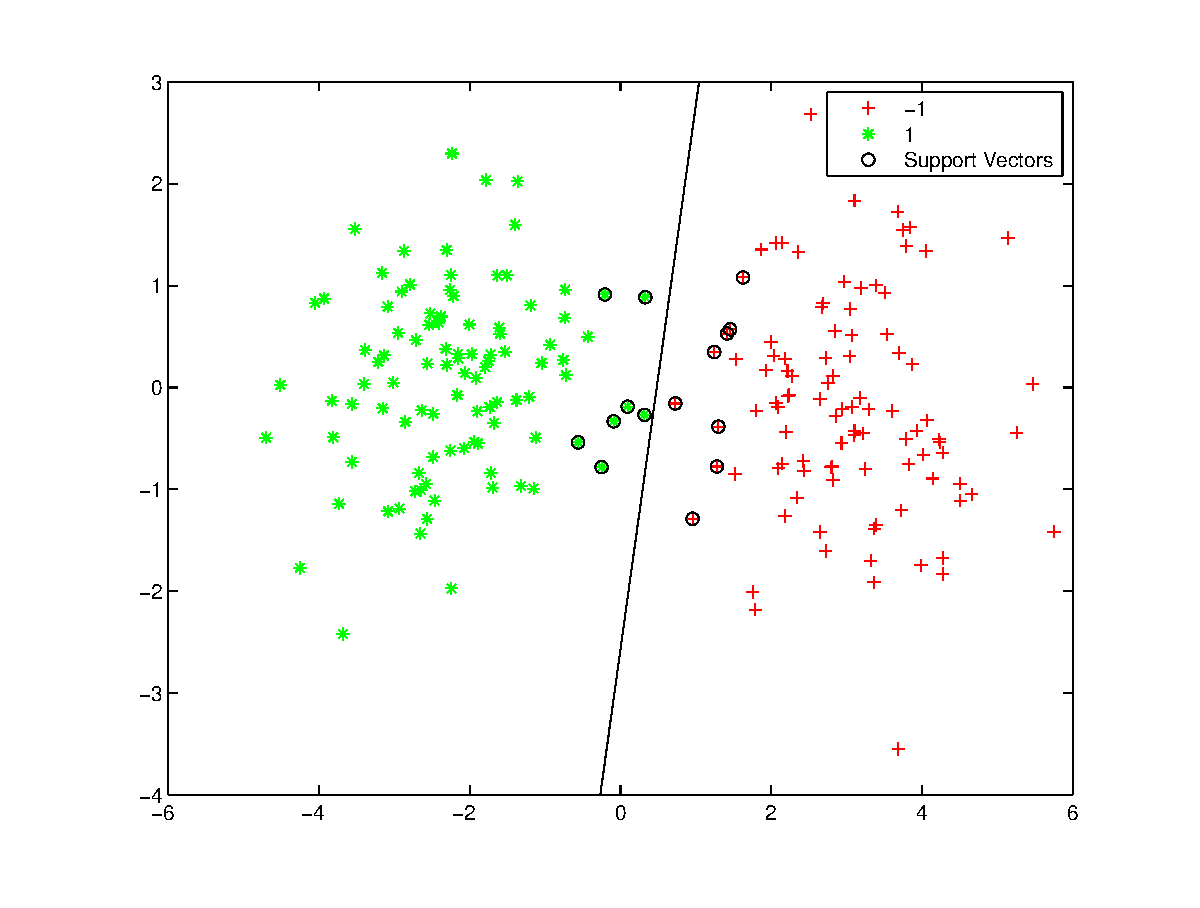
\includegraphics[width=0.8\textwidth]{svm_linear_classification.eps}
    \caption{Classification using a linear kernel SVM}
    \label{fig:svm_linear_classify}
\end{figure}

\begin{figure}[t]
    \centering
    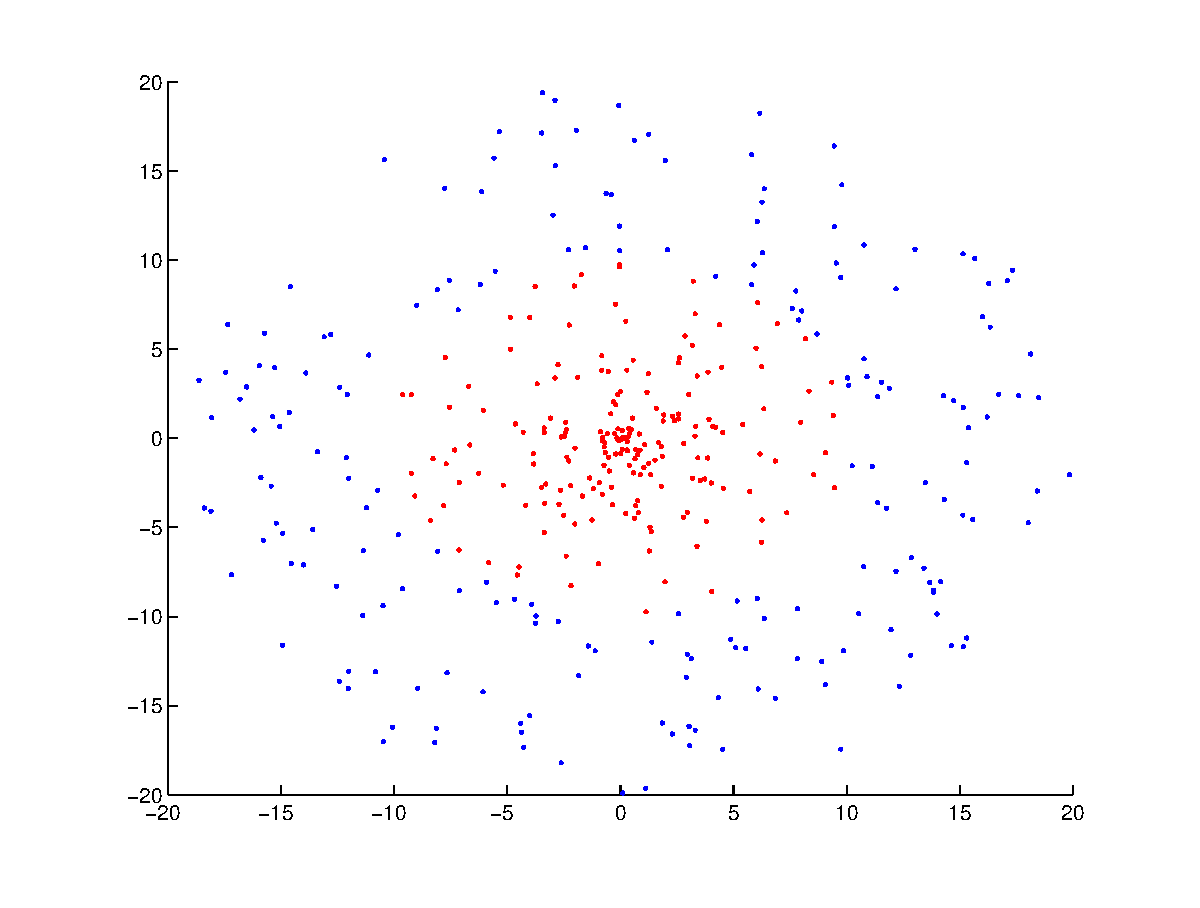
\includegraphics[width=0.8\textwidth]{svm_non_linear_data.eps}
    \caption{A dataset which is not linearly separable}
    \label{fig:svm_non_linear_data}
\end{figure}

\begin{figure}[t]
    \centering
    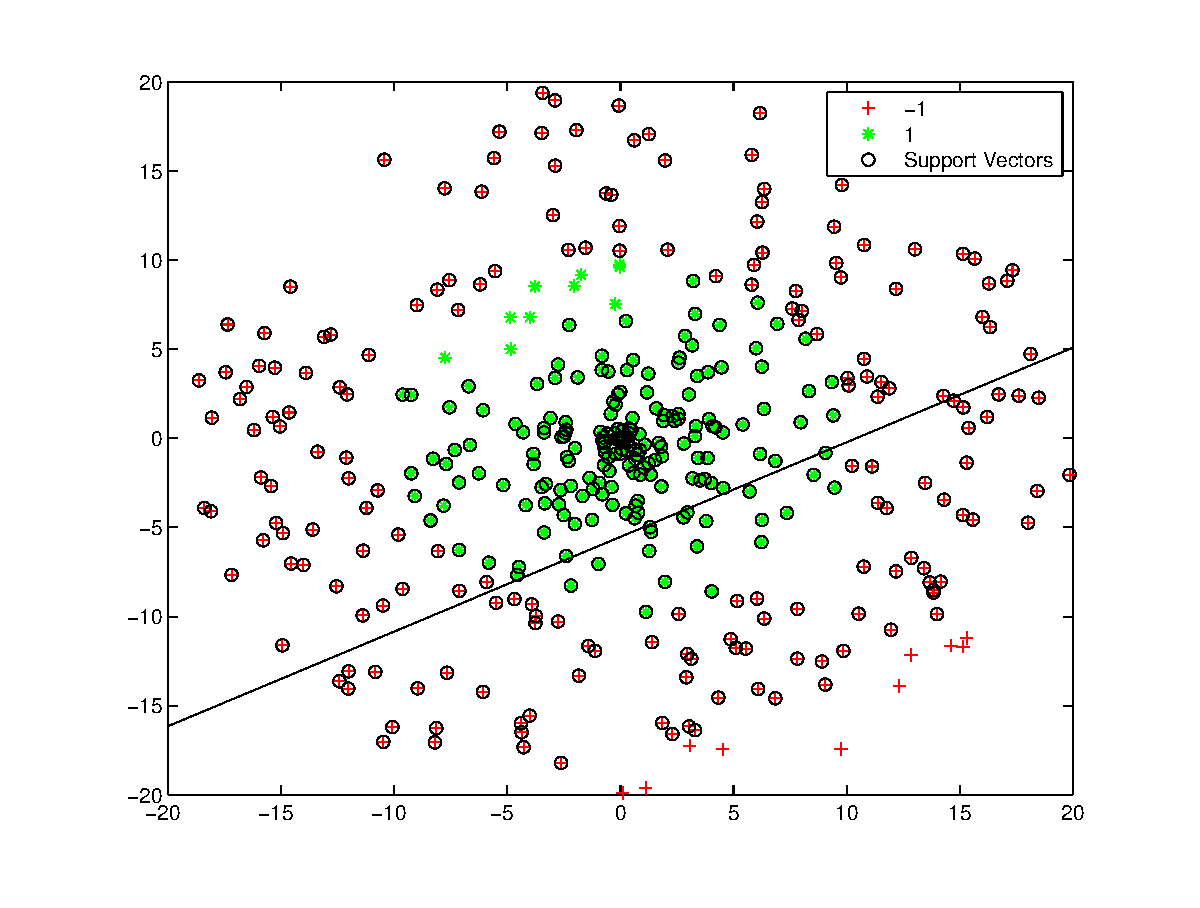
\includegraphics[width=0.8\textwidth]{svm_non_linear_classify_linear.eps}
    \caption{Dataset for Figure~\ref{fig:svm_non_linear_data} being classified using a linear kernel}
    \label{fig:svm_non_linear_classify_linear}
\end{figure}

\begin{figure}[t]
    \centering
    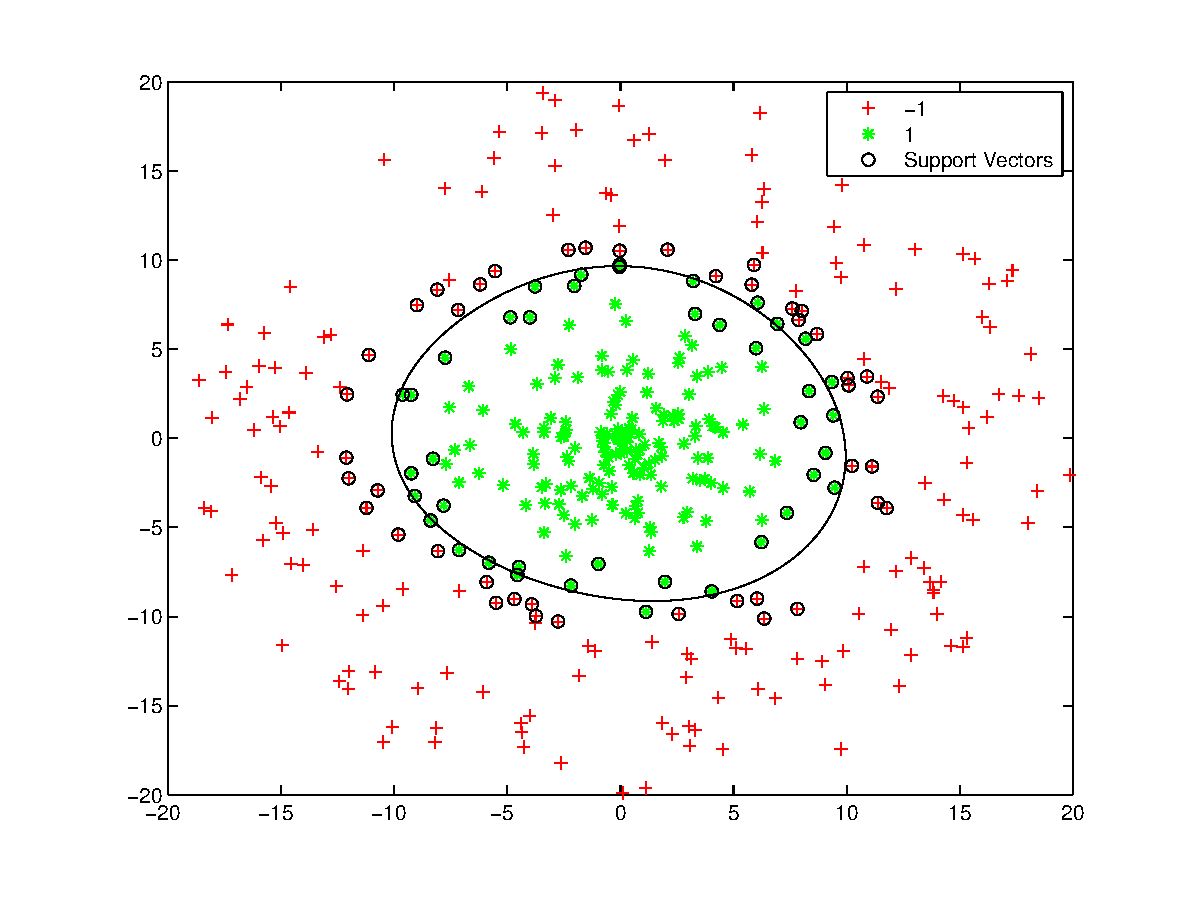
\includegraphics[width=0.8\textwidth]{svm_non_linear_classify_rbf.eps}
    \caption{Dataset for Figure~\ref{fig:svm_non_linear_data} being classified using an RBF kernel}
    \label{fig:svm_non_linear_classify_rbf}
\end{figure}

The most popular kernel functions include
\begin{itemize}
    \item{Linear (the simple SVM) - $\mathbf{K(x, y)} = (\mathbf{x} \cdot \mathbf{y})$ }
    \item{Polynomial - $\mathbf{K(x, y)} = (\gamma \mathbf{x} \cdot \mathbf{y} + \mathbf{c})^{\mathbf{d}}$}
    \item{Radial Basis - $\mathbf{K(x, y)} = \exp(-\gamma {| \mathbf{x} - \mathbf{y} |}^{2})$}
    \item{Sigmoid - $\mathbf{K(x, y)} = \tanh(\gamma \mathbf{x} \cdot \mathbf{y} + \mathbf{c})$}
\end{itemize}
